\documentclass[12pt]{article}
\usepackage[letterpaper,margin=2cm,includehead,nomarginpar,headheight=2cm]{geometry}
\usepackage{amsmath,amssymb,fancyhdr,graphicx,xcolor, array, ragged2e, makecell, enumitem, subcaption, adjustbox}
\usepackage{newpxtext,newpxmath,hyperref,sectsty,lastpage,soul, algorithm,algpseudocode,multirow}
\hypersetup{breaklinks=true, pdfauthor={Bryan Adams}, colorlinks=true, citecolor=gmu-green, urlcolor=gmu-green, linkcolor=gmu-coral, pdfborder={0 0 0}}
\definecolor{gmu-green}{RGB}{30,98,56}
\definecolor{gmu-gold}{RGB}{226,168,43}
\definecolor{gmu-coral}{RGB}{243,112,33}

\algnewcommand\cFor{\textbf{For }}
\algnewcommand\eFor{\textbf{ }}

\newcolumntype{M}[1]{>{\centering\arraybackslash}m{#1}}


\title{\sc Work unit evolution: Using large language models to determine temporal task evolution}
\author{Bryan Adams}

\date{December 7, 2023}

\begin{document}
\maketitle

\section*{Abstract}

The proposed research is intended to develop a modeling framework to better understand how working groups within an organization, specifically Army Acquisitions, evolve over time. The research will focus on how a working group's skills, knowledge and abilities (SKAs) evolve over a given period. The modeling approach will require research into identifying what qualifies as a SKA, as well as, identifying and implementing methods to identify SKAs consistently within unstructured Army Acquisitions’ job postings, which is a set of free text documents. The research will provide the ability to create sets of required SKAs for a given acquisition team $j$ at period $t$, $\Omega_t^j$. Sets $\Omega_t^j$, will enable the creation of a modeling framework with the purpose of modeling an organization's working groups temporal evolution as it relates to SKAs.

\section{Introduction}

Understanding required knowledge, skills, and abilities (KSAs) required for a vacancy is essential in understanding individual career progression. As an individual moves from one position to another, they learn new KSAs or advanced their current capabilities. Comprehending an individual's KSAs evolution and career progression is necessary for gaining a more comprehensive understanding of the economy. Understanding how an employee's KSA evolves overtime enables a better understanding how a firm and industry evolves. 

Analyzing individual KSAs evolution and career progression is difficult as it evolves analyzing a variety of data sources and interactive components. There is the formal education and training and individual receives, the informal on-the-job training, and the development of techniques learned through social interaction of their work unit within an organization. Unfortunately, no organization records data which encompasses all data necessary for understanding individual KSAs evolution as a member of an organization transitions from one position to another. Understanding individual KSAs evolution will enable the creation of a modeling framework with the purpose of modeling an organization's individual and working groups temporal evolution in order to better forecast vacancies and individual career transitions. 

To date there does not exist a framework to analyze individual or work unit evolution, nor is there a defined method for measuring the magnitude of the evolution. The majority of previous work focuses on modeling evolution at the firm, industry or country level. Additionally, with respect to KSAs, previous research combines them into a single taxonomy of "tasks." In this paper I analyze methods to create a KSA space necessary to measure the magnitude of the difference between two positions within the Army Acquisitions Workforce (AAW). The KSA space will enable a way to measure an individual's and work unit's KSA evolution to provide the basis of a mathematical model to forecast career progression within an organization.

\section{Related work}

\subsection{Defining KSAs}

A significant amount of work has been focussed on defining KSAs and determining a broad definition of KSA requirements for a general occupation. In the United States, O\textsuperscript{*}NET created and currently maintains occupation specific descriptors. These descriptors created the O\textsuperscript{*}NET content model, which is used to define occupations within Standard Occupational Classification (SOC) system. O\textsuperscript{*}NET, funded by the Department of Labor and Statistics, was formed in order to develop a descriptive system to define occupations. Prior to O\textsuperscript{*}NET, the majority of jobs were defined by required tasks but there was not a common metric available to compare and contrast jobs based on their requirements.\cite{onet_content_model}

O\textsuperscript{*}NET defines a knowledge "as a collection of discrete but related facts and information about a particular do main."\cite{knowledges} By conducting an extensive review of the cognitive, vocational, training, and job analysis literatures, O\textsuperscript{*}NET created 14 knowledge clusters and 49 knowledges.\cite{knowledges} These knowledges provide researches the taxonomy required to develope knowledge requirements for a specific occupation. Example knowledge definitions are found in Table \ref{tab:knowledge_examples}.

Skills makes up an additional component of O\textsuperscript{*}NET's content model. Skills take on a variety of context, as such O\textsuperscript{*}NET defines skills in terms of procedures incorporating the instability of an individual skills, the different levels of generality, and needed to incorporate the method an individual acquires and applies the skill.\cite{skills} O\textsuperscript{*}NET labels skills as Basic, content and process skills, and Cross-functional, problem-solving, social, technical, systems, and resource management skills.\cite{skills}

Lastly, O\textsuperscript{*}NET defines abilities as relatively enduring attributes of an individual's capability for performing a particular range of different tasks.\cite{abilities} An ability is an individual trait related to the quality of work performed when completing a task required for an occupation. O\textsuperscript{*}NET identifies 52 abilities which create the taxonomy for identifying the required abilities required to perform a specific task.\cite{abilities}  

\subsection{Data sources and KSA aggregation}

Extensive research exists in identifying relevant KSAs for specific occupations or industries, but little research exists at identifying KSAs related to a specific vacancy, let alone how the positions KSAs evolve over time. The problem of KSA identification spans multiple research domains and has been extensively researched in economics, management and sociology. \cite{investment_human_capital, task_specific, on_the_mechanics, diversification}. Classifying identified KSAs is also extensively researched in many fields.\cite{specialization_career,industry-specific_human_capital, human_capital_specificity} 

Prior research does not have a consensus on what data sources are optimal for identifying KSAs nor how one should aggregate the required KSAs. Neffke looks at individual's education and work histories for the entire Swedish population.\cite{value_of_complementarity} Although education history is concrete data, it only represents one way an individual acquires KSAs and assumes degrees across multiple universities are equivalent. Similarly, Neffke et al. use data from administrative records that cover roughly 4.5 million individuals who were employed in over 400 different industries in Sweden between 2004 and 2007.\cite{skill_relatedness} However, the data are at an industry level and not individual, work unit, or firm focused. 

Anderson et. al looks at worker profiles and job listings at random from a publicly available website.\cite{anderson2017skill} One is able to identify required KSAs for a job opening based on a job listing; however, their data does not enable them to measure KSA evolution for a specific position. Hosseinioun et al. examens transition resumes and survey data collected by U.S. Bureau of Labor Statistics, which record the importance and intensity of each skill, knowledge, or ability required in detailed occupational categories.\cite{nested_skills} This data allows them to model an individual's career trajectory based on self-professed KSAs; however, they are unable to incorporate the importance of how the individual acquires the KSAs through formal methods or from interacting with members of a work unit.

Prior research highlights the importance of aggregating specific data sources to better understand KSAs associated with occupation, industry, and in few cases, individual career trajectory. We aim to aggregate KSAs identified from job ad descriptions with an individuals career trajectory within a single organization. This enables us to model the informal aspects of how individuals acquire KSAs through social interaction within a work unit. Although previous methods are applicable, new methods must be developed to model the micro-level of data discussed in this paper.
% \subsection{Large Language Models use in KSA}

\section{Data and Methods}

\subsection{USAjobs job ads}

The AAW is required to post job openings on USAjobs. There is a generally acceptable format for creating a job ad, but each subordinate organization is able to deviate from a standard format. As such, the data is semi-structured, but new methods are needed to identify relevant KSAs required for the position. 

In September 2023, USAJobs contained 2,379,956 of historical job ads with position opening dates from September 12, 2012 to May 26, 2027. The majority of the job ads occur between 2017 and 2023, reference Table \ref{tab:job_opening_count} for a count of job ads by year. The following filtering criteria were applied to determine the relevant AAW job ads. The filtering resulted in a possible 75,914 job ads related to AAW with position opening dates from February 01, 2015 to October 22, 2023. The majority of the job ads occur between 2017 and 2023, reference Table \ref{tab:aaw_job_opening_count} for a count of job ads by year. 

\begin{enumerate}[label=\textbf{Step \arabic*:}, left=0pt]
    \item Filter on job ads with a hiring department of \textit{Department of the Army} or \textit{Department of the Defense} reducing the number of jab ads to 772,297.
    \item Search job add for the term \textit{acquisition} reducing the number of job ads to 75,914.
\end{enumerate}

\begin{table}[ht!]
    \centering
    \vspace*{4mm}
    \begin{subtable}[b]{0.4\linewidth}
        \centering
        % \begin{adjustbox}{valign=t}
        \begin{tabular}{cc}
            \Xhline{3\arrayrulewidth}
            Year &   Count \\\Xhline{3\arrayrulewidth}
            2012 &       1 \\
            2013 &       6 \\
            2014 &      23 \\
            2015 &     143 \\
            2016 &    3893 \\
            2017 &  237451 \\
            2018 &  329440 \\
            2019 &  348783 \\
            2020 &  328452 \\
            2021 &  369111 \\
            2022 &  441709 \\
            2023 &  320874 \\
            2024 &      69 \\
            2027 &       1 \\
            \Xhline{3\arrayrulewidth}
        \end{tabular}
        \caption{Historical job posting counts by position opening year}\label{tab:job_opening_count}
    % \end{adjustbox}
    \end{subtable}
    \begin{subtable}[b]{0.4\linewidth}
        \centering
        % \begin{adjustbox}{valign=t}
        \vspace*{4mm}
        \begin{tabular}{cc}
            \Xhline{3\arrayrulewidth}
                Year &  Count\\\Xhline{3\arrayrulewidth}
                2015 &      5\\
                2016 &     39\\
                2017 &   7537\\
                2018 &  12033\\
                2019 &  13087\\
                2020 &  10320\\
                2021 &  11619\\
                2022 &  12567\\
                2023 &   8707\\
            \Xhline{3\arrayrulewidth}
        \end{tabular}
        \caption{Possible AAW historical job posting counts by position opening year}\label{tab:aaw_job_opening_count}
        % \end{adjustbox}
    \end{subtable}
    \caption{Historical job posting counts from USAjobs}\label{tab:usa_jobs}
\end{table}

\subsubsection{Processing and cleaning data}

Data pulled from USAJobs contains multiple unnecessary characters and unnecessary or redundant phrases. Some examples include html tags and references to U.S. federal regulations. In order to make the data more useable, identified unnecessary characters, such as html tags, and unnecessary or redundant phrases were removed from the job ad descriptions. A raw and processed job ad example can be found in Section \ref{sec:job_ad_example}.

\subsection{Identifying KSAs}

Identifying and classifying KSAs is a non-trivial task when analyzing job ads. O\textsuperscript{*}NET's content model provides the taxonomies necessary, but does not provide a robust method for identifying the KSAs within a job ad. An ad may state "Planning and conducting negotiations on price" or "Developing acquisitions strategies" as requirements, but we need to identify which taxonomy these requirements fall in. Further, job ads might have slight wording difference such as "Planning and \textbf{executing} negotiations on price." With the advancement of large language models (LLMs), we now have a new method to identify occupational requirements for a specific position. We propose using Pathways Language Model 2 (PaLM2) as a method for extracting and classifying job ad requirements.

\subsubsection{PaLM2}

Pathways Language Model (PaLM) uses a standard Transformer model architecture similar to the architecture described in \textit{Attention is all you need}.\cite{attention} There are significant changes in how the model weights are optimized. Those changes include the use of SwiGLU activation function, Parallel Layers in each Transformer block, Transformer formulation uses $k$ attention heads, RoPE embeddings instead of absolute or relative position embeddings, and using SentencePiece for vocabulary.\cite{palm} PaLM2 is an update on PaLM but trained on a larger more diverse data set and redesigned for more compute efficiency and contains 540 billion parameters, 118 layers, and 48 attention heads.\cite{palm2} 

\subsubsection{Using PaLM2 to identify KSAs within job ads}

PaLM2 provides a method for extracting KSAs from free-text data, such as job ads. In this paper we propose using PaLM2 as a method for creating required KSA vectors for job ads. An example knowledge vector for a job ad is [Physics, Economics and Accounting, Business and Management, Education and Training, Mathematics, Chemistry, Engineering and Technology]. In order for PaLM2 to identify if a KSA is required you must first inform PaLM2 what the KSA is and how to identify if the KSA is a stated requirement within the job ad. 

To accomplish this must provide a leading text statement, a query (question), how much variance you want between candidate answers, and the text to search. Example prompts and queries are in Section \ref{sec:palm_prompt}. The variance in response allowed is referred to as temperature. Temperature is set between $[0,1]$. When temperature is 0, your responses are deterministic, while at 1 you will have significant variance in your responses and a higher probability of hallucinations. 

For each query we receive three candidate responses, if each candidate response is a "yes" we add the knowledge to the knowledge vector, reference Section \ref{sec:palm_response} for an example response. After each query is conducted we are have a knowledge vector associated with the job ad, but we do not have a mathematical method for representing the job ads knowledge vector. For this we introduce the KSA space.

\subsection{KSA space}

In order to compare job ad knowledge vectors, we must first define a vector space, KSA space, to measure the distance between two knowledge taxonomies. How different are two knowledges be, for example Administration and Management and Administration, when O\textsuperscript{*}NET provides different definitions? This is necessary to not only measure how different two vacancies are, but to measure how the position evolves overtime. Figure \ref{fig:change} contains a representation of a knowledge vector change over time. Hypothetically, at period $t$ a job requires [Engineering and Technology, Mathematics], at $t+m$ the job requires [Engineering and Technology, Physics] and at $t+n$ the job now requires [Business and Management, Economics and Accounting]. There should be more significant difference between $t+m$ and $t+n$ than $t$ and $t+m$, but how much larger should it be?

Multiple studies demonstrated the ability for embedding models to represent relationships between words and their context within a vector space.\cite{domain_sepcific_words, word_phrases}. Bidirectional Encoder Representations from Transformers (BERT), as an encoder model that has been widely used to perform a variety of natural language processing tasks to include semantic similarity. To create our KSA space we analyze three methods, BERT base uncased, a fine-tuned BERT model, and Sentence-BERT (SBERT).

\begin{figure}[ht!]
    \centering
    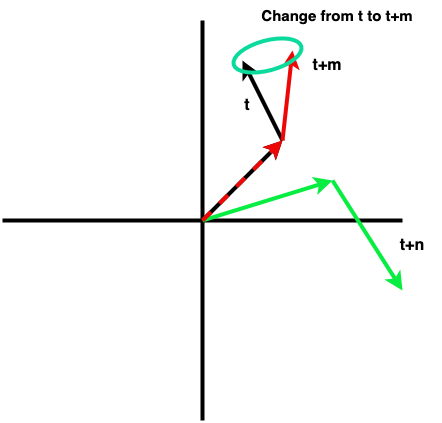
\includegraphics[width=0.4\textwidth]{images/task_change_w_time.png}
    \caption{Representation of job KSA vector changes}
\end{figure}\label{fig:change}

\subsubsection{BERT}

BERT is a multi-layer bidirectional Transformer encoder, whose Transformer architecture makes fine-tuning BERT inexpensive.\cite{bert} The BERT architecture consists of12 layers, 12 attention heads, 110 million parameters, and has a hidden layer with size 768.\cite{bert} The hidden layer is the vector embedding, $\vec{v}_i$ representation of each word, $i$, in a sentence. The embedding layer defines the vector space for each word. Past research has demonstrated, conducting a mean-pooling, equation \ref{eq:mean_pool} of the word embedding vectors provides a vector representation of the sentence with the same dimension 768.\cite{labor_space, sbert}

\begin{equation}
    \text{mean pooling} = \frac{1}{n}\sum_{i=0}^n \vec{v}_i
    \label{eq:mean_pool}
\end{equation}

\subsubsection{Fine-tuning BERT}

As stated perviously, BERT is designed to be fine-tuned for specific tasks or languages with low cost. BERT provides the base weights for one to fine-tune based on their specific context. Since O\textsuperscript{*}NET uses specific language when defining their KSA taxonomies, one would expect a fine-tuned BERT model to create a more representative vector space to compare our KSA vectors. To fine-tune BERT, we first created a vocabulary dictionary using a WordPiece algorithm. WordPiece was developed to better handle rare words that appear in text; however, it can be used to develope a custom vocabulary dictionary to tokenize your specific text\cite{wordpiece}, An example of tokenized text can be found in Section \ref{sec:wordpiece}.

Each knowledge definition is tokenized and 15\% of the tokens are masked to create the training dataset to fine-tune the BERT model, reference Section \ref{sec:wordpiece} for example tokenized and masked sentence. The training data is broken into a batch size of 16. The BERT model is fine-tuned with two epochs and using Adam to optimize the weights with learning rate, $\alpha = 0.00005$, hyper-parameters $\beta_1 = 0.9$, $\beta_2 = 0.98$, and correcting for initialization bias.\cite{kingma2017adam}

\subsubsection{SBERT}

SERT was developed using BERT base uncased and adding an additional pooling layer with the objective of increase BERTs performance at determine which sentence pairs are similar (should be close in vector space) and which pairs are dissimilar (should be far away in vector space).\cite{sbert} SBERT was fined-tuned after adding a mean pooling layer and using sentence pairs where the similarity was computed using the cosine similarity, equation \ref{eq:cos_sim}, between the two embeddings, $\vec{u},\vec{v}$.\cite{sbert}

\begin{equation}
    cos\theta = \frac{\vec{u} \cdot \vec{v}}{\|\vec{u}\|\|\vec{v}\|}
    \label{eq:cos_sim}
\end{equation}

\section{Resulting KSA space}

BERT, fine-tuned BERT, and SBERT where used to create vector embedding for each O\textsuperscript{*}NET knowledge definition. The projected representations of each vector embedding are in Figure \ref{fig:ksa_space}. Each knowledge is colored by their general O\textsuperscript{*}NET defined categories. Visually  in two-dimensions, it appears all three models provide adequate results by clustering categories relatively close together; however, it does not help answer if they are an adequate distance apart based on their definitions.

\begin{figure}
    \centering
  
    \begin{subfigure}{0.45\textwidth}
      \centering
      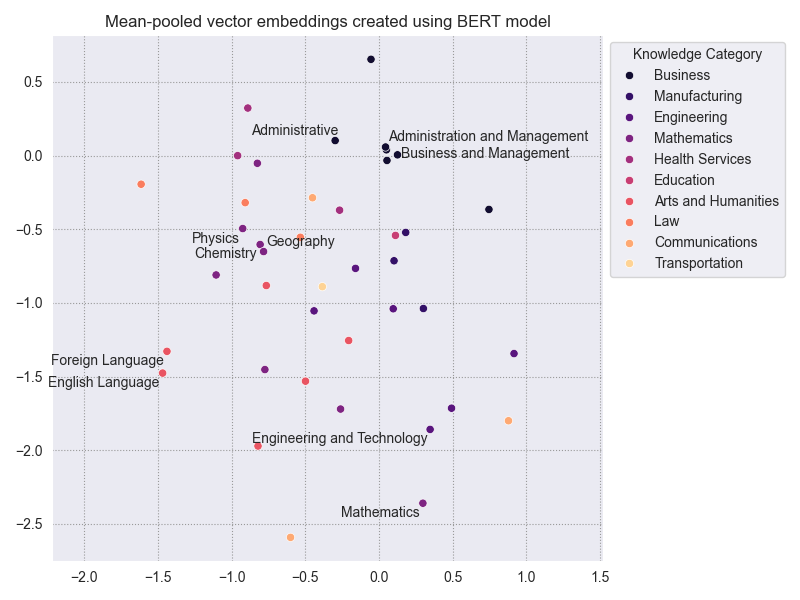
\includegraphics[width=\linewidth]{../plots/base_bert.png}
      \caption{BERT base uncased vector embeddings projection}
      \label{fig:ksa_space_base_bert}
    \end{subfigure}
    \hfill
    \begin{subfigure}{0.45\textwidth}
      \centering
      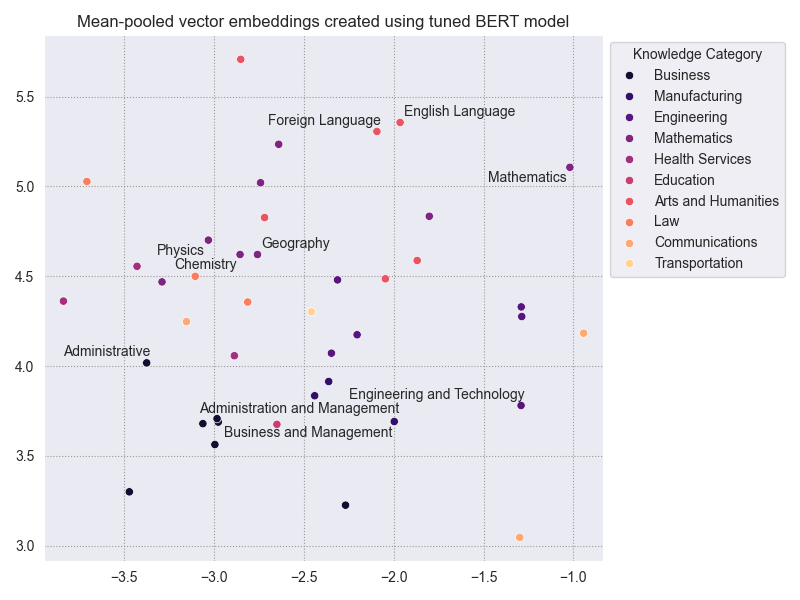
\includegraphics[width=\linewidth]{../plots/tuned_bert.png}
      \caption{Tuned BERT vector embeddings projection}
      \label{fig:ksa_space_tuned_bert}
    \end{subfigure}
  
    \vspace{10pt} % Adjust the vertical space between rows
  
    \begin{subfigure}{0.45\textwidth}
      \centering
      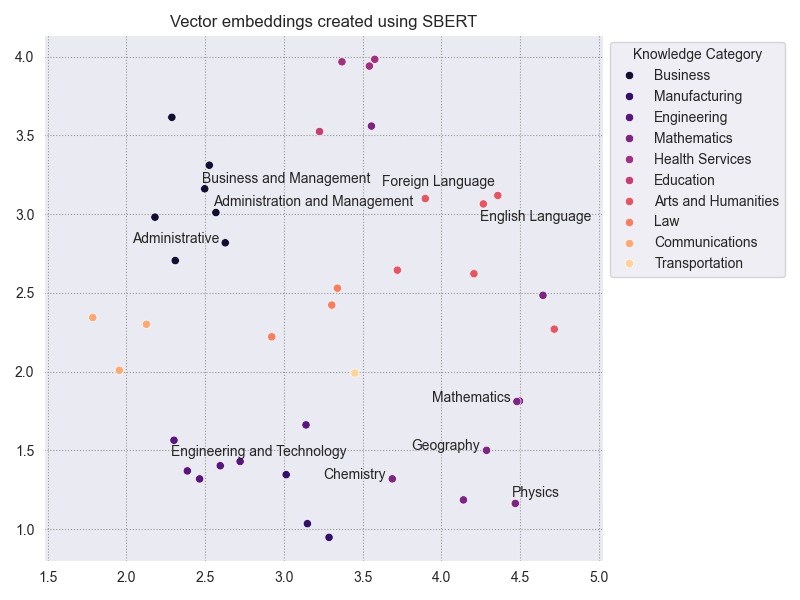
\includegraphics[width=\linewidth]{../plots/base_sbert.png}
      \caption{SBERT vector embeddings projection}
      \label{fig:ksa_space_sbert}
    \end{subfigure}
  
    \caption{Projected knowledge space created using BERT based uncased, Tuned BERT, and SBERT}
    \label{fig:ksa_space}

\end{figure}

\section{Comparing KSAs}

We calculated the cosine similarity between pairs of knowledge definitions using BERT, fined-tuned BERT and SBERT created vector embeddings to compare how different two knowledge definitions are. Table \ref{tab:ksa_compare_methods} contains the cosine similarities between selected paris of knowledges. Both BERT and fine-tune BERT have similar similarity scores and they are higher than the SBERT. This might be preferable when you are comparing knowledges within the same knowledge category, for example Buisinees and Management with Administration and Management. SBERT appears to do a better job in measuring the difference between knowledges in different categories, for example Mathematics and English.\\

\begin{table}[ht!]
    \centering
    \vspace*{-6mm}
    \begin{tabular}{m{5.5cm}m{5.5cm}M{1cm}M{1cm}M{1cm}}
        \Xhline{3\arrayrulewidth}
        \multicolumn{1}{m{5.5cm}}{\centering Element 1}& 
        \multicolumn{1}{m{5.5cm}}{\centering Element 2} & 
        \multicolumn{1}{m{1cm}}{\centering SBERT} & 
        \multicolumn{1}{m{1cm}}{\centering Tuned BERT} & 
        \multicolumn{1}{m{1cm}}{\centering BERT base} \\\Xhline{3\arrayrulewidth}
        Business and Management & \raggedright Administration and Management & 0.731 & 0.859 & 0.865 \\\hline
        \raggedright Administration and Management & Administrative & 0.336 & 0.759 & 0.782 \\\hline
        Mathematics & Physics & 0.264 & 0.719 & 0.742 \\\hline
        Engineering and Technology & Mathematics & 0.277 & 0.727 & 0.732 \\\hline
        Administrative & Mathematics & 0.203 & 0.702 & 0.722 \\\hline
        English Language & Foreign Language & 0.831 & 0.941 & 0.965 \\\hline
        Mathematics & English Language & 0.170 & 0.706 & 0.724 \\
        \Xhline{3\arrayrulewidth}
    \end{tabular}
    \caption{Cosine similarity between knowledge descriptions}\label{tab:ksa_compare_methods}
\end{table}
  
\section{Discussion and future work}

\begin{itemize}
    \item PaLM2 prompt generation - providing more specificity in prompt will increase validity of response, e.g. add examples of misclassification to the prompt
    \item Determine the optimal model to use to define the vector space of KSAs
\end{itemize}
  

\clearpage

\section{Supplemental material}

\subsection{Example O\textsuperscript{*}NET knowledges}

\begin{table}[ht!]
    \centering
    \vspace*{4mm}
    \begin{tabular}{c | >{\RaggedRight} m{10cm}} 
        \Xhline{3\arrayrulewidth}
        Element name & Element definition \\\hline\hline
        Administration and Management & Knowledge of business and management principles involved in strategic planning, resource allocation, human resources modeling, leadership technique, production methods, and coordination of people and resources. \\
        Administrative & Knowledge of administrative and office procedures and systems such as word processing, managing files and records, stenography and transcription, designing forms, and workplace terminology. \\
        Mathematics & Knowledge of arithmetic, algebra, geometry, calculus, statistics, and their applications. \\
        Engineering and Technology & Knowledge of the practical application of engineering science and technology. This includes applying principles, techniques, procedures, and equipment to the design and production of various goods and services. \\
        \Xhline{3\arrayrulewidth}
    \end{tabular}
    \caption{O\textsuperscript{*}NET example knowledges and definitions}\label{tab:knowledge_examples}
\end{table}

\newpage

\subsection{USAJobs ad data}

\subsubsection{USAJobs ad data fields}

\begin{table}[ht!]
    \centering
    \vspace*{4mm}
    \begin{tabular}{c | >{\RaggedRight} m{10cm}} 
        \Xhline{3\arrayrulewidth}
            Source & \multicolumn{1}{>{\centering}p{10cm}}{Data fields} \\ \hline\hline
            Historical job metadata &  USAJobsControlNumber, hiringAgencyCode,hiringAgencyName, hiringDepartmentCode, hiringDepartmentName,agencyLevel, agencyLevelSort, appointmentType, workSchedule,payScale, salaryType, vendor, travelRequirement,teleworkEligible, serviceType, securityClearanceRequired,securityClearance, whoMayApply, announcementClosingTypeCode,announcementClosingTypeDescription, positionOpenDate,positionCloseDate, positionExpireDate, announcementNumber,hiringSubelementName, positionTitle, minimumGrade, maximumGrade,promotionPotential, minimumSalary, maximumSalary,supervisoryStatus, drugTestRequired, relocationExpensesReimbursed,totalOpenings, disableAppyOnline, positionOpeningStatus,applicationsStarted, hiringPaths, jobCategories,positionLocations, missionCriticalOccupations,keyStandardRequirements, \_links \\\hline
            Historical job text & USAJobsControlNumber, positionOpenDate, positionCloseDate,summary, hiringPathExplanation, duties, majorDutiesList,requirementsConditionsOfEmployment, requirementsQualifications,requirementsEducation, requiredStandardDocuments,requiredDocuments, howToApply, howToApplyNextSteps,requirements, evaluations, benefitsURL, benefits,otherInformation, appointmentTypeOverride,positionScheduleOverride, exclusiveClarificationText, videoURL \\\hline
            Job add webpage & uic, address \\
        \Xhline{3\arrayrulewidth}
    \end{tabular}
    \caption{USAjobs ad data fields by source}\label{tab:job_fields}
\end{table}
  
\subsubsection{Example USA job ad descriptions}\label{sec:job_ad_example}

\textbf{Raw job ad:}\\

To qualify for a Contract Specialist your resume and supporting documentation must support: $<$br /$>$\textbackslash n$<$br /$>$\textbackslash nA. . Basic DoD 1102 Requirement: Public Law 106-398, Section 808: A.) A baccalaureate degree from an accredited educational institution authorized to grant baccalaureate degrees AND B.) at least 24 semester hours (or equivalent) of study from an ... Creditable specialized experience includes:$<$br /$>$\textbackslash n$<$br /$>$\textbackslash nGS-13:\textbackslash n$<$ul$>$\textbackslash n \textbackslash t$<$li$>$Developing contractual strategies.$<$/li$>$\textbackslash n \textbackslash t$<$li$>$Ensuring acquisition plans are in full compliance with contracting regulations and related Department of Defense (DoD) standards.$<$/li$>$\textbackslash n \textbackslash t$<$li$>$Planning and conducting negotiations on price, technical requirements, terms, and conditions of the contract.$<$/li$>$\textbackslash n \textbackslash t$<$li$>$Developing acquisitions strategies and/or determining methods of procurement and ensuring proper performance.$<$/li$>$\textbackslash n$<$/ul$>$\textbackslash nGS-12:\textbackslash n\textbackslash n$<$ul$>$\textbackslash n \textbackslash t$<$li$>$Verifies for accuracy purchase requests, prepares acquisition plans, conducts market research and recommends contract type and pricing strategies.$<$/li$>$\textbackslash n \textbackslash t$<$li$>$Performs price and cost analysis, analyzing unit costs and pricing data and contractors projected costs.$<$/li$>$\textbackslash n \textbackslash t$<$li$>$Performs full range of contract administration functions.$<$/li$>$\textbackslash n \textbackslash t$<$li$>$Assists with extensive negotiations which address acquisition related issues with offerors.$<$/li$>$\textbackslash n \textbackslash t$<$li$>$Assists to prepare and issue contract modifications under long term contracts.$<$/li$>$\textbackslash n \textbackslash t$<$li$>$Assists in developing contractual strategies.$<$/li$>$\textbackslash n \textbackslash t$<$li$>$Develops cost and price analysis spreadsheets for long-term contracts.$<$/li$>$\textbackslash n$<$/ul$>$\textbackslash nE...\\

\noindent \textbf{Cleaned job ad:}\\

To qualify for a Contract Specialist your resume and supporting documentation must support: A baccalaureate degree from an accredited educational institution authorized to grant baccalaureate degrees AND B.) at least 24 semester hours (or equivalent) of study from an ... Creditable specialized experience includes:GS-13:Developing contractual strategies.Ensuring acquisition plans are in full compliance with contracting regulations and related Department of Defense (DoD) standards.Planning and conducting negotiations on price, technical requirements, terms, and conditions of the contract.Developing acquisitions strategies and/or determining methods of procurement and ensuring proper performance.GS-12:Verifies for accuracy purchase requests, prepares acquisition plans, conducts market research and recommends contract type and pricing strategies.Performs price and cost analysis, analyzing unit costs and pricing data and contractors projected costs.Performs full range of contract administration functions.Assists with extensive negotiations which address acquisition related issues with offerors.Assists to prepare and issue contract modifications under long term contracts.Assists in developing contractual strategies.Develops cost and price analysis spreadsheets for long-term contracts.

\newpage

\subsection{Pathways Language Model 2 (PaLM2)}

\subsubsection{Example PaLM2 prompt}\label{sec:palm_prompt}

\textbf{Leading text provided to PaLM2}\\

\noindent $<$knowledge name$>$ is the $<$knowledge description$>$. Look at the job ad and decide if $<$knowledge name$>$ is required to perform this job. If $<$knowledge name$>$ is required please provide the specific tasks in a bulletized format from the job ad that relate to $<$knowledge name$>$, if not simply say no.\\

\noindent \textbf{Query provided to PaLM2}\\

\noindent Does this job ad require $<$knowledge name$>$ knowledge to perform the job?

\subsubsection{Example PaLM2 response}\label{sec:palm_response}

\textbf{Example response for job ad in Section \ref{sec:job_ad_example}}\\

Candidate 1: Yes.

The job ad requires the following skills:

\begin{itemize}
  \item Knowledge of Federal and agency contracting laws and regulations applicable to centralized acquisition of agency-wide commodity and service requirements
  \item Knowledge of commercial business and industry practices and trends, cost factors, and market conditions along with understanding the military support requirements to be procured to identify potential contractors in limited supplier source situations.
  \item Developing of pre-negotiation plans, negotiation techniques, and cost and price analysis of procurement proposals to independently decide on proper strategies to procure complex requirements.
  \item Applying negotiation, persuasion and compromise techniques is required to negotiate price, terms and conditions, delivery schedule, contract modifications, (quantity options and extension of contract performance periods) and settlement of contractor claims in the best interest of the Government.
\end{itemize}

\clearpage

\subsection{WordPiece and sentence tokenization}\label{sec:wordpiece}

\textbf{Tokenized knowledge description}

\begin{verbatim}
    ['[CLS]', 'principles', 'and', 'facts', 'related', 'to', 'business', 
    'administration', 'and','accounting', ',', 'human', 'and', 'material', 
    'resource', 'management', 'in', 'organizations', ',', 'sales', 'and', 
    'marketing', ',', 'economics', ',', 'and', 'office', 'information', 
    'and', 'organizing', 'systems', '[SEP]', '[PAD]', ...]
\end{verbatim}
    


\textbf{Whole word masking}

\begin{verbatim}
    ['[CLS]','[MASK]','and','[MASK]','related','to','business',
    '[MASK]','and','accounting',',','human','and','[MASK]',
    'resource','management','in','organizations',',','sales','and',
    'marketing','[MASK]','economics','[MASK]','and','office','information',
    'and','organizing','systems','[SEP]','[PAD]'...]
\end{verbatim}


\textbf{WordPiece tokenizing}

\begin{verbatim}
    [['[CLS]','principle','\#\#s','and','facts','related','to','business',
    'administration','and','accounting',',','human','and','material',
    'resource','management','in','organizations',',','sales','and',
    'marketing',',','economics',',','and','office','information',
    'and','organizing','systems','[SEP]']]
\end{verbatim}





\clearpage

\bibliographystyle{plain}
\bibliography{refs}

\end{document}

